% 2007 年上海卷文科第 21 题：“果圆”与两椭圆焦点、坐标轴交点。
% 取满足 a^2=b^2+c^2、b>c>0 的示意参数；曲线形状和坐标比例均不代表题设定值。
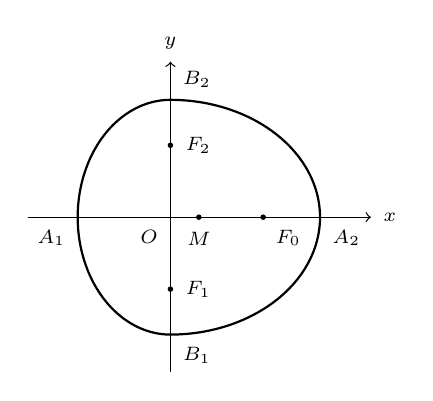
\begin{tikzpicture}[x=1.9cm,y=1.9cm,line cap=round,line join=round,
  line width=.45pt,every node/.style={font=\scriptsize}]
  \pgfmathsetmacro{\a}{1}
  \pgfmathsetmacro{\c}{.62}
  \pgfmathsetmacro{\b}{sqrt(\a*\a-\c*\c)}
  \pgfmathsetmacro{\f}{sqrt(\b*\b-\c*\c)}
  \pgfmathsetmacro{\m}{(\a-\c)/2}

  \draw[->] (-.95,0)--(1.34,0) node[right=1pt] {$x$};
  \draw[->] (0,-1.03)--(0,1.04) node[above=1pt] {$y$};

  \draw[thick,domain=-90:90,samples=100,variable=\t]
    plot ({\a*cos(\t)},{\b*sin(\t)});
  \draw[thick,domain=90:270,samples=100,variable=\t]
    plot ({\c*cos(\t)},{\b*sin(\t)});

  \fill (\m,0) circle (1pt);
  \fill (\c,0) circle (1pt);
  \fill (0,\f) circle (1pt);
  \fill (0,-\f) circle (1pt);

  \node[below left=1pt] at (-\c,0) {$A_1$};
  \node[below right=1pt] at (\a,0) {$A_2$};
  \node[below left=1pt] at (0,0) {$O$};
  \node[below=2pt] at (\m,0) {$M$};
  \node[below right=1pt] at (\c,0) {$F_0$};
  \node[above right=1pt] at (0,\b) {$B_2$};
  \node[below right=1pt] at (0,-\b) {$B_1$};
  \node[right=2pt] at (0,\f) {$F_2$};
  \node[right=2pt] at (0,-\f) {$F_1$};
\end{tikzpicture}
